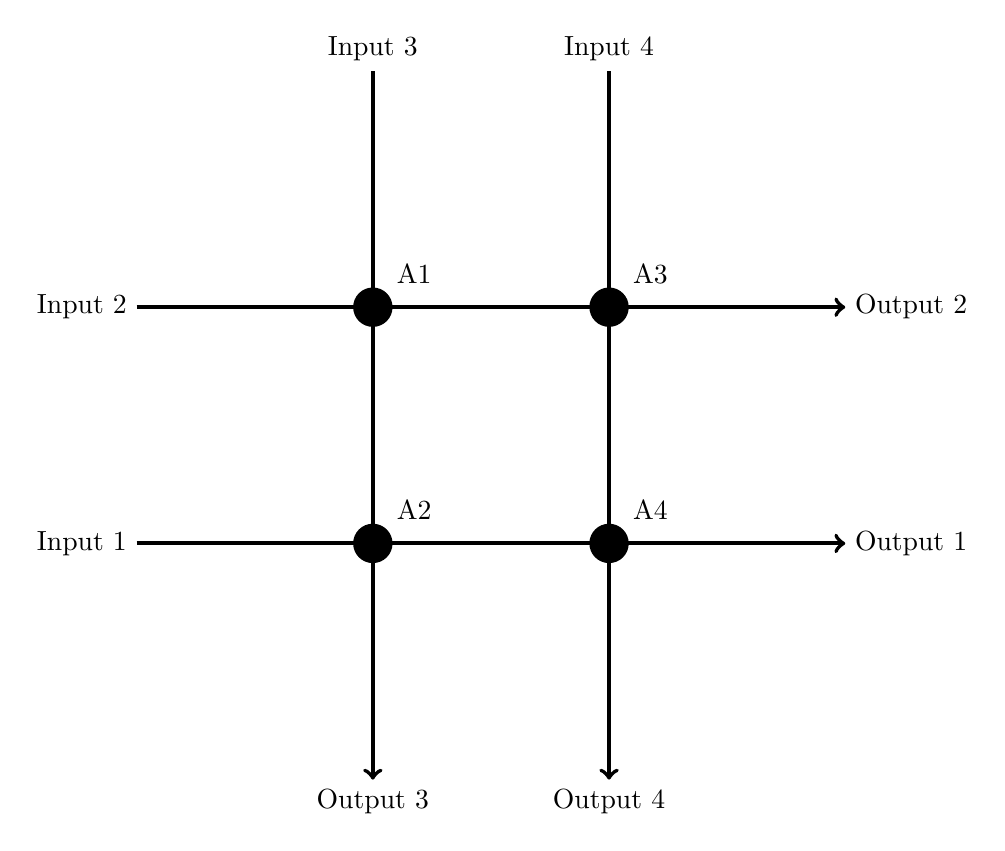
\begin{tikzpicture}
	\draw[->, line width = 1.5] (-3,0) -- (6,0);
	\draw[->, line width = 1.5] (-3,3) -- (6,3);
	\draw[<-, line width = 1.5] (0,-3) -- (0,6);
	\draw[<-, line width = 1.5] (3,-3) -- (3,6);

	\node at (-3,0) [left] {Input 1};
	\node at (-3,3) [left] {Input 2};
	\node at (0,6) [above] {Input 3};
	\node at (3,6) [above] {Input 4};

	\node at (6,0) [right] {Output 1};
	\node at (6,3) [right] {Output 2};
	\node at (0,-3) [below] {Output 3};
	\node at (3,-3) [below] {Output 4};

	\node at (0,3)  [circle,fill=black,minimum size=.5cm,label=above right:A1] {};
	\node at (0,0)  [circle,fill=black,minimum size=.5cm,label=above right:A2] {};
	\node at (3,0)  [circle,fill=black,minimum size=.5cm,label=above right:A4] {};
	\node at (3,3)  [circle,fill=black,minimum size=.5cm,label=above right:A3] {};
\end{tikzpicture}